\documentclass[11pt]{article}
%\usepackage{fullpage}
\usepackage[top=2cm, bottom=1.5cm, left=1.5cm, right=1.5cm]{geometry}
\usepackage{amsmath,amsthm,amsfonts,amssymb,amscd}
\usepackage{xcolor}
\usepackage{graphicx}
\usepackage[utf8]{inputenc}
\usepackage[english]{babel}
\usepackage{fancyhdr}
\usepackage{wrapfig}

\pagestyle{fancy}
\fancyhf{}
\fancyhead[LO]{Mechanics \& Relativity F3210}
\fancyhead[RO]{Workshop 5: Forces Part 2}
%\fancyfoot[CE,CO]{\leftmark}
%\fancyfoot[LE,RO]{\thepage}

%answers
\usepackage{etoolbox}
\providetoggle{answers}
\settoggle{answers}{false}

\newcommand\vect[1]{\underline{\mathbf{#1}}}
\newcommand\unitvect[1]{\hat{\boldsymbol{#1}}}

\begin{document}

\noindent
\textbf{\textcolor{red}{Please upload your solution to Problem 3 to canvas for marking after the workshop.}}\\

\section*{Problem 1}

In downhill speed skiing a skier is retarded by both the air drag force on the body and the kinetic frictional force on the skis. Suppose the slope angle is $\theta = 40.0^{\circ}$, the snow is dry snow with a coefficient of kinetic friction $\mu_k = 0.0400$, the mass of the skier and equipment is $m = 85.0$ kg, the cross-sectional area of the (tucked) skier is $A = 1.30$ m$^2$, the drag coefficient is $C = 0.150$, and the air density is 1.20 kgm$^{-3}$. \\
(a) What is the terminal speed? \\
(b) If a skier can vary C by a slight amount dC by adjusting, say, the hand positions, what is the corresponding variation in the terminal speed?\\


\noindent

\section*{Problem 2}

A box of sugar ($m_s = 1.0$ kg) and a box of flour ($m_f = 3.0$ kg) are accelerated across a horizontal surface by a horizontal force $\vect{F}$ applied to the sugar box. The magnitude of the frictional force on the sugar box is 2.0 N, and the magnitude of the frictional force on the flour box is 4.0 N. If the magnitude of $\vect{F}$ is 12 N, what is the magnitude of the force on the flour box from the sugar box?


\section*{\textcolor{red}{Problem 3}}
\fbox{\begin{minipage}{\textwidth}
The graph below shows the spring force $F_{x}$ versus position x for the spring-block arrangement in the figure. The scale is set by $F_s = 160.0$~N. We release the block at x = 12 cm. 
(a) How much work does the spring do on the block when the block moves from $x_i = +8.0$~cm to $x_f = +5.0$~cm? 
(b) from $x_i = +8.0$~cm to $x_f = -5.0$~cm? 
(c) from $x_i = +8.0$~cm to $x_f = -8.0$~cm? 
(d) from $x_i = +8.0$~cm to $x_f = -10.0$~cm?
\end{minipage}}
\begin{figure}[h]
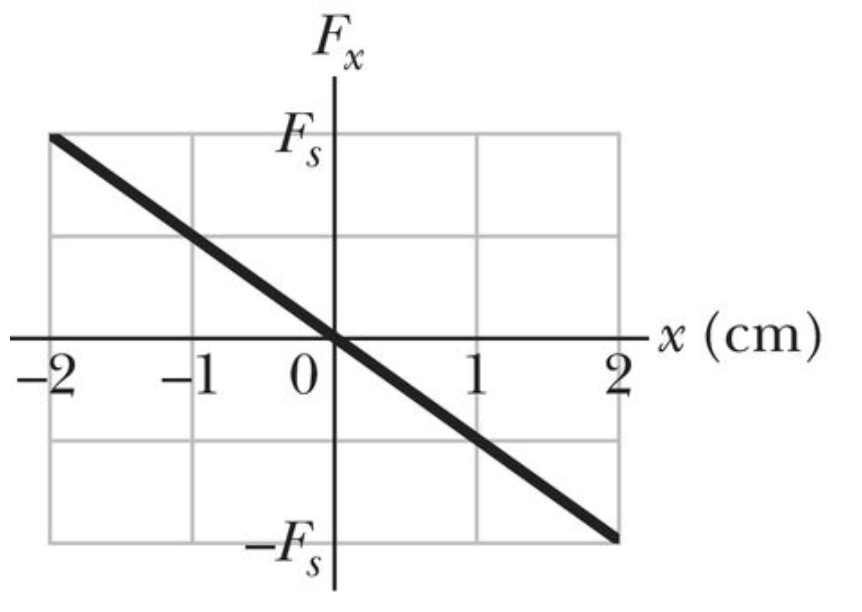
\includegraphics[scale=0.5]{2021-W5-Q3}
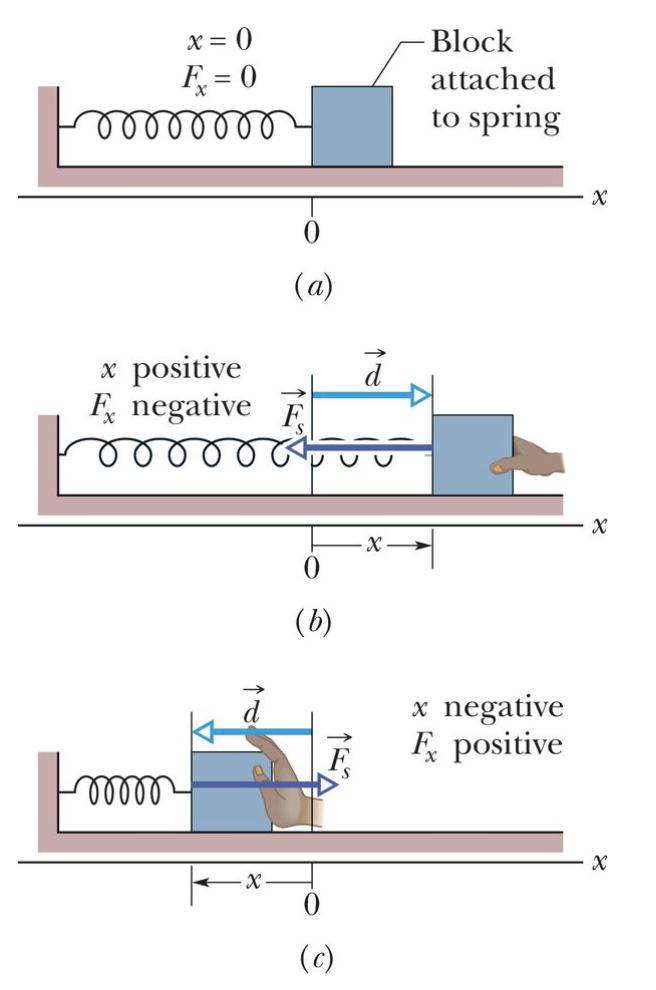
\includegraphics[scale=0.4]{2021-W5-Q3-2}
\end{figure}

%\vspace{0.5cm}
\section*{Want more practice?}
\small
Further problems on Friction \& Drag: Chapter 6.1,6.2 \\
Further problems on KE: Chapter 7.1,7.2 \\
Further problems on Springs \& Gravity: Chapter 7.3,7.4 \\
\end{document}





 




 


